\documentclass[a4paper,11pt]{article}

\usepackage[slovene]{babel}
\usepackage[utf8]{inputenc}

\usepackage{listings}
\usepackage{babelbib}
\usepackage{url}

\usepackage{graphicx}
\graphicspath{ {images/} }

\usepackage{underscore}
\renewcommand{\lstlistingname}{Primer}% Listing -> Primer

\lstset{
numbers=left, 
numberstyle=\small, 
numbersep=8pt, 
frame = single, 
language=Python, 
framexleftmargin=15pt}

\setlength{\parindent}{0pt}
%BORDERS
\usepackage{geometry}
 \geometry{
 a4paper,
 total={170mm,257mm},
 left=30mm,
 right=25mm,
 top=30mm,
 bottom=30mm
 }

\begin{document}
\begin{titlepage}


% ZAČETNA STRAN
\newcommand{\HRule}{\rule{\linewidth}{0.5mm}} % Defines a new command for the horizontal lines, change thickness here

\center % Center everything on the page
 
%----------------------------------------------------------------------------------------
%	HEADING SECTIONS
%----------------------------------------------------------------------------------------

\textsc{ UNIVERZA V MARIBORU\\ FAKULTETA ZA ELEKTROTEHNIKO,\\RAČUNALNIŠTVO IN INFORMATIKO}\\[5cm] % Name of your university/college

%----------------------------------------------------------------------------------------
%	TITLE SECTION
%----------------------------------------------------------------------------------------
{ \huge \bfseries \textbf{ZAČETEK SPRINTA 4}}\\[0.4cm] % Title of your document
\textsc{\large Povezljivi sistemi in inteligentne storitve}\\[5cm] % Minor heading such as course title

%----------------------------------------------------------------------------------------
%	AUTHORS SECTION
%----------------------------------------------------------------------------------------
{\large Gašper Gračner}\\[0.4cm]
{\large Martin Oprešnik}\\[0.4cm]
{\large Luka Koštomaj}\\[0.4cm] 

%----------------------------------------------------------------------------------------
%	DATE SECTION
%----------------------------------------------------------------------------------------
\vfill % Fill the rest of the page with whitespace
{\large Maribor, Maj 2016}\\[3cm] % Date, change the \today to a set date if you want to be precise
\end{titlepage}
\newpage

%----------------------------------------------------------------------------------------
%	CONTENT SECTION
%----------------------------------------------------------------------------------------

\section{Predvidene naloge}
V drugem sprintu smo si vsi zadali analizo oz. testiranje izbranih metod strojnega učenja.
	\begin{enumerate}
		\item{Gašper Gračner- Uporaba različnih implementacij SVM,}
		\item{Luka Koštomaj - Izboljšava napovedi nevronske mreže,}
		\item{Martin Oprešnik - klasifikacija treningov}
	\end{enumerate}
	
\begin{figure}[h]
\caption{Zaslonska slika odprtih nalog}
\centering
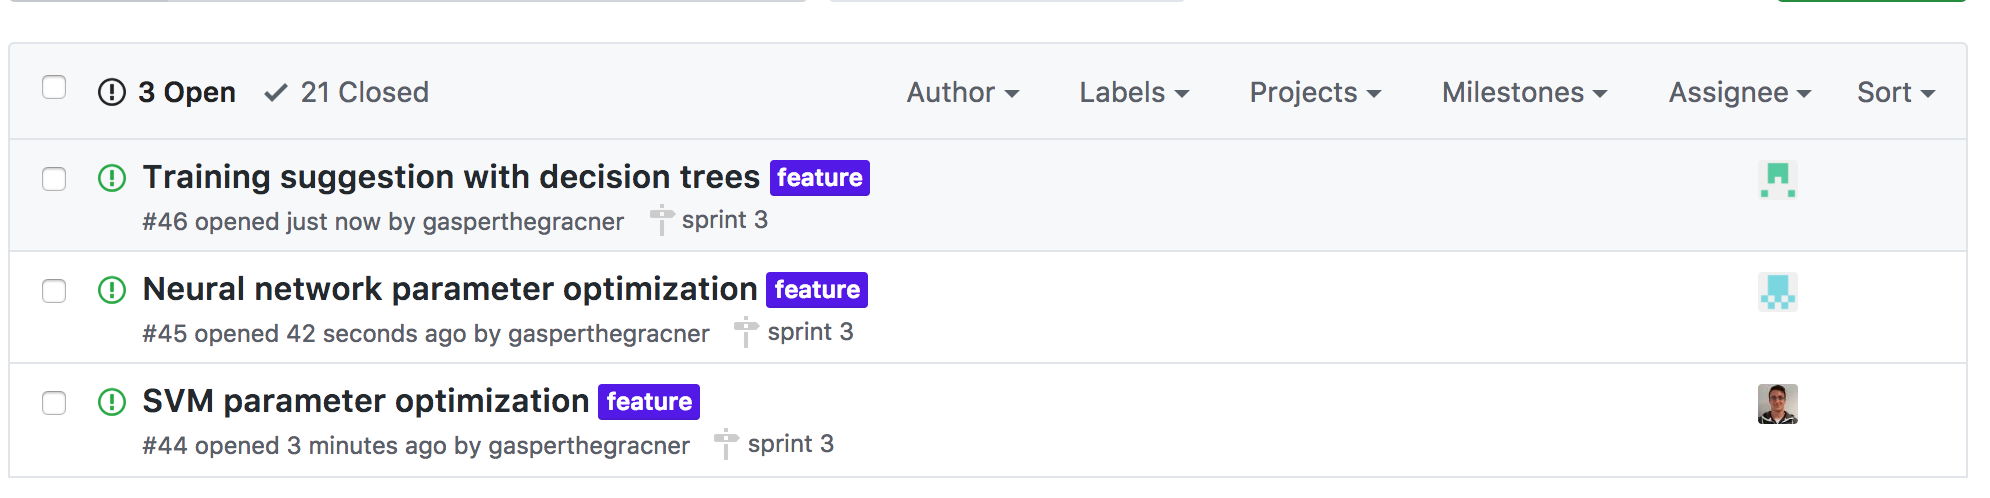
\includegraphics[width=1\textwidth]{issues}
\end{figure}

\newpage
\section{Gašper Gračner- Uporaba različnih implementacij SVM}
Sodeloval bom pri implementaciji metode priporočanja treningov.
Na koncu, bom poskusal uporabiti in primerjati še različne klasifikatorje, ki podpirajo SVM
in so implementirani v uporabljeni knjižnici (SVC, NuSVC in LinearSVC). Moral pa bom
določiti tudi primerno metodo primerjanja klasifikatorjev. 

\section{Luka Koštomaj - Izboljšava učenja nevronske mreže}

Na koncu, bom testiral nevronsko mrežo in s tem poskušal spremeniti testno množico, da bi mogoče izboljšalo napoved.

\section{Martin Oprešnik - klasifikacija treningov }

V tem sprintu bom poskusil uporabiti naučeno drevo odločitev, tako da se zgenerira več kombinacij treninga, ki se klasificirajo v razrede. Izhod bodo treningi, ki so se klasificirali najvišje.




\end{document}